% ----------------------------------------------
\chapter{INTRODUÇÃO}\label{cap:introducao}
% ----------------------------------------------
A base para o desenvolvimento de um sistema de monitoramento digital capaz de acompanhar produtos perecíveis, passa por um entendimento de todos os elos envolvidos. Dentre eles a dinâmica entre a temperatura e o crescimento de vida microbiana (Listeria) bem como a logística nacional para esse tipo de alimento. Além disso, deve-se considerar também as limitações técnicas para o desenvolvimento de dispositivos IoT capazes de obter dados críticos de todo o processo.
%\section{Contexto do Ambiente}
%%%%%%%%%%%%%%%%%%%%%%%%%%%%%%%%%%%%%%%%%%%%%%%%%%%%%%%%%%%%%%%%%%%%%%
\section{Produtos perecíveis}
%%%%%%%%%%%%%%%%%%%%%%%%%%%%%%%%%%%%%%%%%%%%%%%%%%%%%%%%%%%%%%%%%%%%%%
Denominam-se alimentos perecíveis aqueles que possuem uma quantidade significativa de água. Isso os torna vulneráveis a proliferação de vida microbiana que é a principal responsável pela decomposição destes alimentos. Para se manterem conservados, estes alimentos necessitam manter-se refrigerados.
Alimentos perecíveis estão presentes no dia a dia das populações no mundo inteiro, pois muitos deles são a base de uma alimentação saudável devido a pouca exposição a conservantes ou processos industriais que embora eliminem as suas bactérias, acabam por eliminar também os seus nutrientes.
Com o objetivo de mapear a composição dos principais alimentos consumidos no Brasil, a \citeonline{Anvisa2011} desenvolveu o projeto TACO (Tabela Brasileira de Composição de Alimentos). A partir desta, obteve-se um detalhamento da tabela nutricional e demais dados dos alimentos que compõe o dia a dia dos brasileiros.

Com base nisso, apresenta-se um problema relacionado a distribuição destes alimentos ao longo de um país como o Brasil que possui dimensões continentais e alguns alimentos são produzidos apenas em certas regiões.
Com o objetivo de predizer o impacto do aumento de listeria, \citeonline{monica} apresenta um algoritmo baseado em redes neurais artificiais \textit{Multilayer Perceptron} (MLP) em função dos impactos atmosféricos a que esses alimentos são submetidos. A capacidade de prever a vida útil destes alimentos a partir de fatores ambientais pode ser decisivo para a escolha do meio de transporte do mesmo e para o aumento das exigências de qualidade que redes atacadistas impõe no ato de revenda dos mesmos.

%%%%%%%%%%%%%%%%%%%%%%%%%%%%%%%%%%%%%%%%%%%%%%%%%%%%%%%%%%%%%%%%%%%%%%
\section{Logística}
%%%%%%%%%%%%%%%%%%%%%%%%%%%%%%%%%%%%%%%%%%%%%%%%%%%%%%%%%%%%%%%%%%%%%%
Dentro de uma cadeia de distribuição de alimentos, existe uma série de desafios logísticos envolvidos no processo e todos esses processos são responsáveis por um grau de depreciação na vida útil de alimentos como frutas, verduras e legumes (FLV). Analisar essa cadeia é essencial para compreender que quanto mais elementos envolvidos, como intermediários, maior as chances de se perder a rastreabilidade e a qualidade dos FLV.
Os autores \citeonline{Aliotte2022} detalham que os fatores mais importantes a serem observados no processo de distribuição são:
\begin{itemize}
    \item Tipo de transporte
    \item Agente responsável pelo transporte
    \item Rastreabilidade
    \item Acondicionamento em câmara fria
    \item Tipos de embalagem
    \item Troca de embalagem
    \item Manipulação da carga
\end{itemize}

Dentre estes, cabe destaque para o tipo de transporte, que pode ser de caminhão baú frigorificado oferecendo temperaturas abaixo de 0~$^o$C; caminhão baú refrigerado que pode manter temperaturas entre 0~$^o$C e 12~$^o$C; caminhão graneleiro que possui apenas proteção com lona para orvalho, sol e chuva e não possui controle de refrigeração; caminhão baú sem refrigeração que se assemelha ao graneleiro; além do caminhão com carroceria aberta. Na Figura~\ref{fig:transporte} é possível ver a distribuição de uso destes caminhões para alguns tipos de cargas.

\begin{figure}[h!]
  \caption{Transporte por tipo de carroceria.}
  \begin{center}
      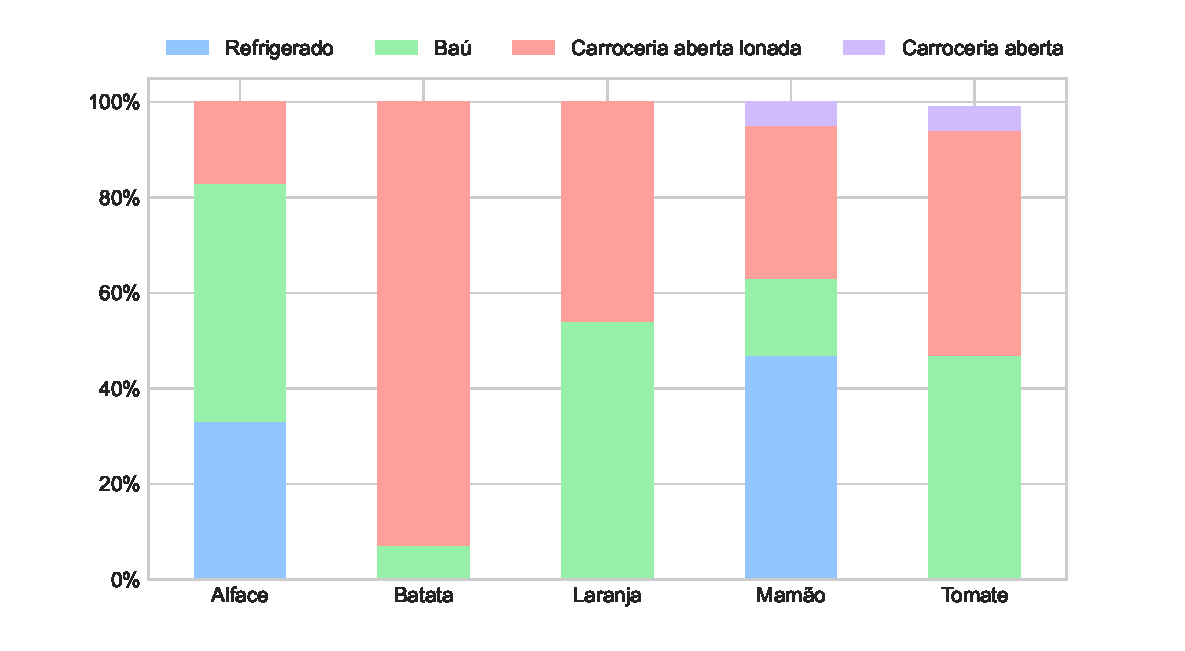
\includegraphics[trim={0 1.2cm 0 0.5cm },scale=0.6]{img/transporte.pdf}
  \end{center}
  \fonte{Elaborado pelo autor com base em~\cite{Aliotte2022} }
  \label{fig:transporte}
\end{figure}
%\Floatbarrier

Uma vez introduzidas as diferentes formas de transporte \citeonline{Aliotte2022} discorrem sobre os agentes responsáveis pelo transporte e suas particularidades. Fatores como distância a ser percorrida e a terceirização do transporte são efetivamente relevantes, impactando diretamente na qualidade dos FLV.

Ao tratar da rastreabilidade e acondicionamento em câmara fria, \citeonline{Aliotte2022} apontam uma demanda do mercado por qualidade. Fica evidente que investimentos nessas áreas possuem um apelo não só para atender consumidores exigentes como normas sanitárias.

Já os três últimos tópicos: tipos de embalagem, troca de embalagem e manipulação da carga, dizem respeito aos impactos da embalagem tanto ao condicionamento como ao desgaste ocasionados no processo de alocação.

``Para que o produto chegue ao destino em boas condições, é necessário que ocorra o mínimo de manuseio, que sejam cumpridas as regras sanitárias nas operações de carga e descarga, além do uso de tecnologias que reduzam a manipulação por ação humana.'' \cite[p.~16]{Aliotte2022}.





%%%%%%%%%%%%%%%%%%%%%%%%%%%%%%%%%%%%%%%%%%%%%%%%%%%%%%%%%%%%%%%%%%%%%%
\section{IoT}
%%%%%%%%%%%%%%%%%%%%%%%%%%%%%%%%%%%%%%%%%%%%%%%%%%%%%%%%%%%%%%%%%%%%%%
O termo \textit{Internet of Things} (IOT), traduzido livremente para ``Internet das Coisas'', popularizou-se nos últimos anos devido aos avanços tecnológicos em termos de miniaturização de circuitos eletrônicos. Graças a esses avanços, um mundo de opções se abriu para resolver problemas que antes eram impossíveis como o controle de iluminação artificial em uma horta apresentado por \citeonline{9268238} que controla um sistema de espelhos para garantir um adequado fornecimento de luz, além de coletar informações disponibilizando-as em uma plataforma web.

Dispositivos IoT tem como princípio básico o acesso direto a internet, seja para apenas enviar informações, apenas receber ou ambos. A principal vantagem desses sistemas se dá em função da possibilidade de externar o processamento, garantindo assim um requisito de hardware mínimo local, deixando tarefas complexas para a rede externa (Nuvem).  

A popularização dos sistemas IoT se dá de forma tão rápida que até mesmo problemas decorrentes da sincronização de dispositivos passam a ser tratados com soluções como a apresentada por \citeonline{7924944}. Já aplicações que perdem a adesão são rapidamente descontinuadas como a solução da empresa Amazon para comprar sabão de roupas com um botão instalado na máquina de lavar segundo \citeonline{amazon} mostrado na Figura~\ref{fig:amazon}.

\begin{figure}[h!]
  \caption{Amazon Dash Button.}
  \begin{center}
      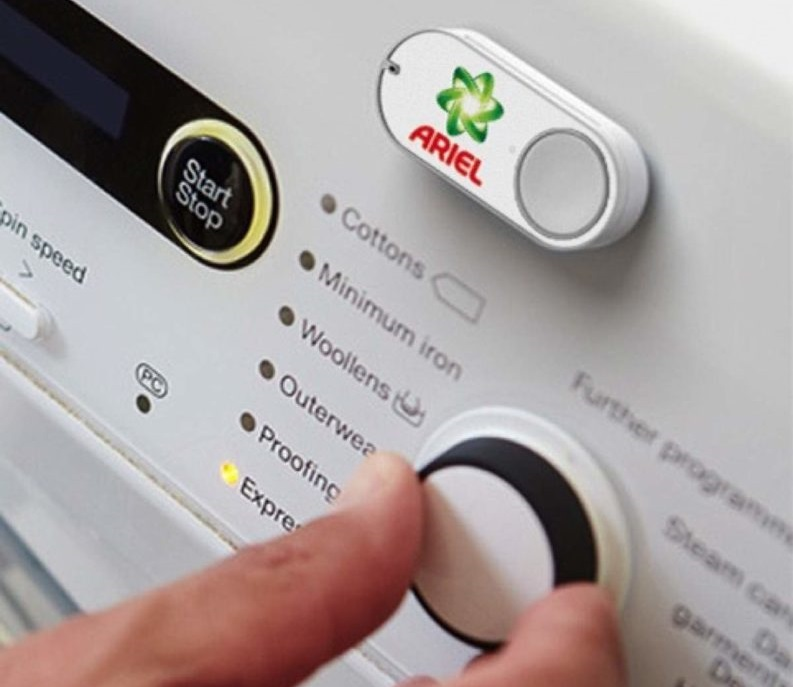
\includegraphics[scale=0.6]{img/Amazon-Dash-Button.png}
  \end{center}
  \fonte{\citeonline{amazondash}}
  \label{fig:amazon}
\end{figure}
%\Floatbarrier

Segundo \citeonline{8648462}, os principais desafios para empregabilidade de sistemas IoT são a extrema heterogeneidade que diz respeito aos diferentes tipos de dispositivos e protocolos envolvidos, a dinâmica imprevisível que diz respeito aos ambientes distintos e obstáculos físicos além da escalabilidade no núcleo que trata dos problemas que envolvem o acesso de vários dispositivos a uma mesma nuvem. Este último, se apresenta como grande relevância para os próximos anos, pois o aumento da quantidade de ``coisas'' ligadas a internet tendem a crescer em demasia.

% ----------------------------------------------
\section{TEMA} 
% ----------------------------------------------
O desenvolvimento de sistema capaz de operar nestas condições e fornecendo dados suficientes para monitorar as condições ambientais como temperatura de transporte requer que a solução possua alguns atributos.

\begin{itemize}
    \item Baixo valor agregado, uma vez que precisa ser empregado em caixas de transporte de alimentos;
    \item Ocupar a menor área possível;
    \item Operar sem a necessidade trocas de pilhas ou recarregamento de baterias;
    \item Traçar um perfil de temperatura com pelo menos uma hora de intervalo entre cada medida;
\end{itemize}
% ----------------------------------------------
\section{DELIMITAÇÃO DO TEMA} 
% ----------------------------------------------
Como proposta de projeto, uma adequação se faz necessária para que a solução eletrônica possa ser conectada a um dispositivo de colheita de energia que embora não seja desenvolvido neste trabalho, levará em consideração suas restrições. Outro aspecto importante é capacidade da solução desenvolvida ser conectada a um dispositivo de \textit{"Wake-up Receiver"} que possibilite a redução do consumo de energia oriundas do trabalho executado por um receptor de rádio constantemente ligado. Devido a essa capacidade de comunicação por rádio, a escolha de um padrão/protocolo de rádio deve ser escolhido.
% ----------------------------------------------
\section{PROBLEMA}
% ----------------------------------------------
Manter a mobilidade de um sistema IoT só é possível com uma solução capaz de transmitir estes dados sem a utilização de fios e cabos. Ao mesmo tempo, a energia necessária para operação destes normalmente é proveniente de baterias. Estas por sua vez possuem muito problemas de depreciação, corrosão e necessidade de compartimentos que muitas vezes são a porta de entrada para umidade. Soma-se a isso o fato de uma verificação da vida útil das mesmas, terá como consequência uma troca futura gerando resíduo eletrônico.

% ----------------------------------------------
\section{OBJETIVOS}
% ----------------------------------------------
Desenvolver uma aplicação de baixo consumo para ser alimentado por um sistema de colheita de energia, dispensando o uso de pilhas ou baterias e poder ser acordado por um sistema de \textit{"Wake-up Receiver"} para transmitir e receber dados por RF somente em situações necessárias. 


% ----------------------------------------------
\section{OBJETIVOS ESPECÍFICOS}
% ----------------------------------------------
\begin{itemize}
    \item Desenvolvimento de um sistema embarcado para aplicação IoT;
    \item Possibilidade de transmitir sinais de rádio frequência;
    \item Armazenar dados em uma memória e cruzar os dados coletados com uma medida de tempo;
    \item Necessitando assim o desenvolvimento de um circuito elétrico;
    \item Uma placa de circuito;
    \item Software capaz de executar todas as funções do sistema;
    \item Encontrar uma solução alternativa ao uso de baterias para a alimentação;
    \item Desenvolvimento deste protótipo funcional;
    \item Avaliação de desempenho energético que deve ser feita para avaliar quanto tempo é necessário para o carregamento através de um dispositivo de colheita de energia.
\end{itemize}
%%%%%%%%%%%%%%%%%%%%%%%%%%%%%%%%%%%%%%%%%%%%%%%%%%%%%%%%%%%%%%%%%%%%%%

%%%%%%%%%%%%%%%%%%%%%%%%%%%%%%%%%%%%%%%%%%%%%%%%%%%%%%%%%%%%%%%%%%%%%%








